\chapter{Zufallsexperimente}
\subsubsection{Beispiele}
\textbf{Werfen einer Münze}\\ Ausgänge: K,Z\\
Grundmenge $\Omega$ = \{K,Z\}\medskip\\
\textbf{Werfen eines Würfel}\\
Ausgänge : 1...6\\
Grundmenge $\Omega$ = \{1,...,6\}\medskip\\
\textbf{Zwei Münzen gleichzeitig werfen}\\
$\Omega$ = \{KK,KZ,ZK,ZZ\}\\
ZK heißt 1. Zeigt Zahl, zweite Kopf. KZ andersherum. Dies gilt wenn die Münzen \textbf{unterscheidbar sind}\medskip\\
\textbf{n Münzen werfen}\\
$\Omega = \{K,Z\}^n = \{(a_1,...,a_n):a_i \in \{K,Z\} \forall i = 1,...,n\}$\\
\#$\Omega = 2^n$\\
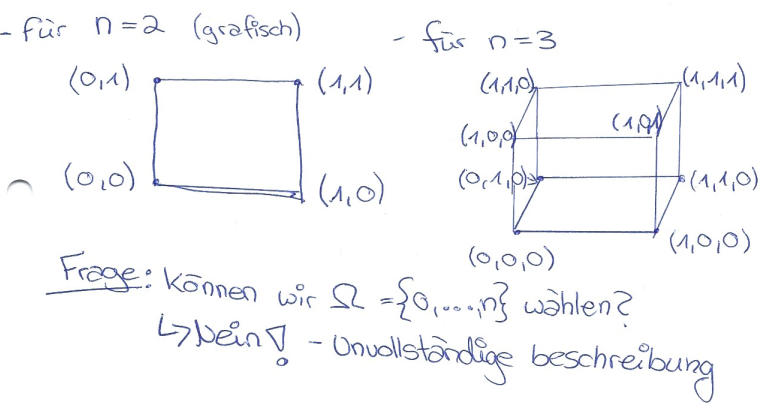
\includegraphics[width=0.8\textwidth]{img/grafikOmega.PNG}
\medskip\\
\textbf{Frage}: Können wir $\Omega = \{0,...,n\}^{n=4}$ wählen?
\section{Produktexperimente}
Betrachte n Experimente mit Grundmengen $E_1,...,E_n$\\
Führe diese Experimente unabhängig voneinander aus.\medskip\\
Grundmenge des Gesamtexperiment ist \\$\Omega = E_1\times ... \times E_n = \{(e_1,...,e_n):e_1 ß\in E_1,...,e_n\in E_n\}$\\
\#$\Omega = \#E_1 \bullet ... \bullet \#E_n$
\subsubsection{Beispiele}
\textbf{Münze und Würfel werfen}
$E_1 = \{K,Z\} \qquad E_2 = \{1,...,6\}$\\
$\Omega = E_1 \times E_2 = $\begin{tabular}{|c|c|c|c|c|c|}
	\hline 
K1	&K2  &K3  &K4  &K5  &K6  \\ 
	\hline 
Z1	& Z2 & Z3 &Z4  &Z5  &Z6  \\ 
	\hline 
\end{tabular} \\
 $\Omega$ = 12
\subsubsection{Definition: Ereignis}
Ereignis = Teilmenge von $\Omega$\\
\textbf{Beispiel}: 1 Würfel. $\Omega$ = \{1,...,6\}\\
Ereignisse: A = ''Würfel zeigt gerade Zahl'' = \{2,4,6\}\\
B = 'Primzahl gewürfelt' = \{2,3,5\}\medskip\\
\textbf{Interpretation}: Zufallsexperiment wird ausgeführt $\Rightarrow$ \\
Wir erfahren den Ausgang w $\in \Omega$\\
Sei A $\subset \Omega$. Liegt w $\in$ A, so sagen wir ''A ist eingetreten''. \\
w $\notin$ A $\Rightarrow$ ''A nicht eingetreten''\medskip\\
\textbf{Beispiel}: 2 Würfel. $\Omega = {1,...,6}^2$\\
A = ''Augensumme  = 10'' = \{(6,4),(5,5),(4,6)\}\medskip\\
Unmögliches Ereignis: $\emptyset$\\
Sicheres Ereignis (tritt immer ein) = $\Omega$\newpage
\section{Boole'sche Algebra}
Seien A $\subset \Omega$; B $\subset \Omega$\\
A $\cup$ B = \{w $\in$ $\Omega$ : w $\in$ A oder w $\in$ B\}\\
= ''mindestens ein Ereignis tritt ein.''\\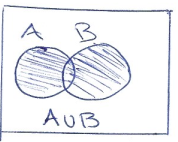
\includegraphics[width=0.2\textwidth]{img/ver.PNG}\medskip\\
A $\cap$ B = \{w $\in$ $\Omega$ : w $\in$ A und w $\in$ B\}\\
= ''beide Ereignisse treten ein.''.\\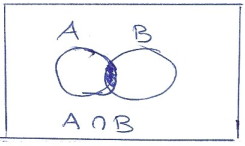
\includegraphics[width=0.2\textwidth]{img/schnitt.PNG}\medskip\\
$A^C =\{ w \in \Omega : w \notin A\}$\\
= ''A tritt nicht ein''\\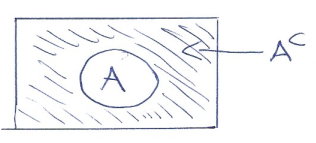
\includegraphics[width=0.3\textwidth]{img/komplement.PNG}\medskip\\
A$\backslash$B = $\{w \in \Omega : w \in A $ und $w \notin B\}$\\
= ''A tritt ein \textbf{und} B tritt nicht ein'' = $A\cap B^C$\medskip\\
B$\backslash$A = $B\cap A \subset$\\
A$\Delta$B = (A$\backslash$B)$\cup$(B$\backslash$A)\\
= ''\textbf{genau} ein Ereignis tritt ein''\\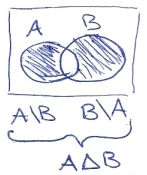
\includegraphics[width=0.2\textwidth]{img/genau1.PNG}\medskip\\
\textbf{Beispiel}: 2 Würfel $\Omega = \{1,...,6\}^2$\\
A = ''1. Würfel zeigt 6 '' = \{(6,1),(6,2),(6,3),(6,4),(6,5),(6,6)\}\\
B = ''2. Würfel zeigt 6'' = Das gleiche, nur vertauscht\medskip\\
A $\cap$ B = \{(6,6)\}\\
A $\cup$ B = \{(6,1),...,(6,6),(1,6),...,(5,6)\}
A $\Delta$ B = \{(6,1),...,(6,5),...,(1,6),...(5,6)\}\newpage
\textbf{Definition: Disjunkt}\\
Ergebnis A und B sind disjunkt, wenn A $\cap$ B = $\emptyset$\\D.h. A und B können nicht gleichzeitig eintreten.\\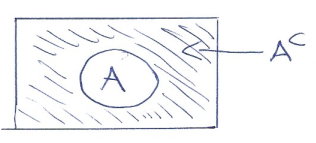
\includegraphics[width=0.3\textwidth]{img/komplement.PNG}\medskip\\
\textbf{Beispiel}: A und $A^C$,\\ A$\backslash$B,\\ A$\Delta$B,\\ und A$\cap$B sind disjunkt.\medskip\\
\textbf{Definition}: A $\subset$ B, wenn $\forall w \in A \Rightarrow w \in B$\\Wenn A eintritt, dann tritt auch B ein.\\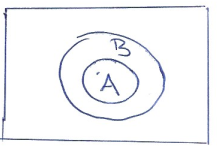
\includegraphics[width=0.3\textwidth]{img/subset.PNG}\medskip\\
\section{De Morgan-Regeln}
$\left( A \cup B\right)^C$ = ''Kein Ereignis tritt ein'' = ''A tritt nicht ein \textbf{und} B tritt nicht ein'' = $A^C \cap B^C$\\
\textbf{Regel}:$(A\cup B)^C = A^C \cap B^C$\medskip\\
$(A \cap B)^C =$''\textbf{mindestens} ein Ereignis tritt nicht ein.'' = ''A tritt nicht ein \textbf{oder} B tritt nicht ein.'' = $A^C\cup B^C$\medskip\\
\textbf{Regel}: ($A\cup B)^C$\\
\textbf{Allgemein}: \\$(A_1\cup,A_2,\cup,...)^C = A_1^C\cap A_2^C\cap...$\\
$(A_1\cap,A_2,\cap,...)^C = A_1^C\cup A_2^C\cup...$
\section{Wahrscheinlichkeiten}
\textbf{Buffon}:\\
4040 Würfe einer Münze. 2048 Kopf.\medskip\\
\textbf{Pearson}: 24000 Würfe, 12012 Kopf\medskip\\
\textbf{Rechner}:100000 Würfe, 50106 Kopf. Häufigkeit: 0,50106\\
\subsection{Empirisches Gesetz der großen Zahlen}
Betrachte Zufallsexperiment und Ereignis A $\subset \Omega$\\
Wiederhole das Experiment n Mal.\\
Zähle, wie oft A eingetreten ist: $kn(A)$ $$\frac{k_n(A)}{n} (\text{Häufigkeit}) \underset{n\rightarrow \infty}{\rightarrow} \mathds {P}[A] \text{(Wkeit von A0)}$$ 
\textbf{Definition}: Diskr. Wahrscheinlichkeitsraum ist ein Paar ($\Omega$,p), wobei $\Omega$ eine Menge ist und
$$:\Omega \rightarrow [0,1] \text{ mit } \sum_w\in \Omega p(w) = 1$$
Wahrscheinlichkeit eines Ausgangs w $\in$ Sigma ist p(w)\\
Wahrscheinlichkeit eines Ereignis A $\subset \Omega : \mathds {P}[A]=\Sigma_{w\in A}\:p(w)$\medskip\\
\textbf{Definition} Ein Laplace-Experiment liegt vor, wenn 
$$\#\Sigma = n < \infty \text{ und } p(w) = \frac{1}{n}\forall w \in \Omega[\text{Ausgänge sind gleichwahrscheinlich}]$$
Dann gilt : $$\mathds {P}[A]=\frac{\#A}{n}= \frac{\#A}{\#\Omega}$$
\textbf{Beispiel}: 2 \textbf{faire} Würfel $\Omega = \{1,...,6\}^2 \qquad \#\Omega = 36$\\
A = ''Augensumme  = 10'' = \{(6,4),(5,5),(4,6)\}
$$\mathds {P}[A] = \frac{3}{36}=\frac{1}{12}$$
B = ''Augensumme = 11'' = \{(6,5),(5,6)\} $\rightarrow \mathds {P}=\frac{1}{18}$\medskip\\
\textbf{Beispiel}: Nicht-Laplace-Experiment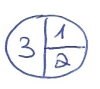
\includegraphics[width=0.1\textwidth]{img/torte.PNG}\\
$\Omega = \{1,2,3\} \qquad p(1) = \frac{1}{4} \quad p(2)=\frac{1}{4} \quad p(3) = \frac{1}{2}$\\oder
$\Omega = \{1,2,3A,3B\} \Rightarrow \text{Laplace-Experiment, da} \\ p(w) = \frac{1}{4} \forall w. \mathds {P}[3] = \frac{1}{4}+\frac{1}{4} = \frac{1}{2}$\medskip\\

